\subsection{BONUS: Compensated Horner's method}
This section contains a Bonus exercice on the Compensated Horner's Method.
The goal is to demonstrate how Verificarlo can be used to compare different evaluation methods and how it interact with numerical functions available through library calls.
 

"Compensated" algorithms belongs to the class of algorithms that increase
program precision without changing the internal working format. 
The goal is to capture for each operation an estimation of the error term and to reinject it into the result.
For the Horner scheme, it is possible to retrieve at every step the error in
$x^2$ and the addition of the next coefficient by using respectively the
$Veltkamp-Dekker$ ({\tt twoProd}) for the product and $twoSum$ for the sum.
These algorithm are qualified as ({\it Error Free Transform}), EFT, in the
literature. 
The algorithm for the compensated horner scheme described in \cite{graillat2005compensated} is:

\begin{algorithmic}[1]
  \Procedure{compHorner}{$x$,$\{a_1, a_2, \ldots, a_n\}$}
    \State {$s_n \gets a_n$}
    \State {$r_n \gets 0$}
    \For {$i \in [n-1:0]$}
       \State $[p_i, pe_i] \gets \text{\sc TwoProd}(s_{i+1}, x^2)$
       \State $[s_i, se_i] \gets \text{\sc TwoSum}(p_i, a_i)$
       \State $r_i \gets r_{i+1}\times x^2+(pe_i+se_i)$
    \EndFor
    \State \Return $s_0 + r_0$
  \EndProcedure
\end{algorithmic}

The lines 5 and 6, evaluates HORNER with EFT calls. Line 7 accumulate the error terms, which will be added to the final result in line 9.

\begin{question}
  \begin{enumerate}[(a)]
    \item Modify {\tt run.sh} to call comphorner with the following command: {\tt ./run.sh COMPHORNER FLOAT 24 }.
  \end{enumerate}
\end{question}

Instead of (carefully) recoding EFTs {\sc TwoProd} and {\sc TwoSum} manually, we suggest to use {\tt libeft}~\cite{libeft} available and documented at the following address: \url{https://github.com/ffevotte/libeft}.

\begin{question}
  \begin{enumerate}[(a)]
    \item Modify {\tt run.sh} to add libeft to the linker command. For this, just add {\tt -left} to verificarlo command and ensure that libeft path is in your  {\tt LIBRARY\_PATH}.
    \item Modify {\tt tchebychev.c} following that example:

      {
      \begin{lstlisting}[style=customC, basicstyle=\normalsize]
      #include <libeft.h>

      /* Define real type and format string */
      #ifdef DOUBLE
      #define REAL double
      #define FMT "%.16e %.16e"
      #define TWOPROD twoprod_d
      #define TWOSUM  twosum_d
      #else
      #define REAL float
      #define FMT "%.7e %.7e"
      #define TWOPROD twoprod_s
      #define TWOSUM  twosum_s
      #endif
      \end{lstlisting}
      }

     These modifications allow defining two macros corresponding to  {\tt TWOPROD} and {\tt TWOSUM} calling the EFT version according to the floating point format you are using.


    \item Implement {\tt REAL compHorner(REAL x)} in {\tt tchebychev.c} according to the comphorner algorithm provided in this tutorial. Modify the {\tt main} function to allow calling comphorner.
    \end{enumerate}
\end{question}


\begin{question}
  Evaluate {\tt compHorner} precision with Verificarlo. What happens if you use a precision different from 53 for program compiled in DOUBLE precision?

  $\Rightarrow$ WARNING, {\sc TwoProd} and {\sc TwoSum} relies on exact operations; it is essential to use RR 53 (Random Rounding with precision 53) mode of verificarlo for  \texttt{double} or RR 24 for \texttt{float}.
  \\~\\
  You should get the results of figures~\ref{fig:comphornerVerificarlo24_53}.
\end{question}


\begin{table}
\begin{tabular}{cc}
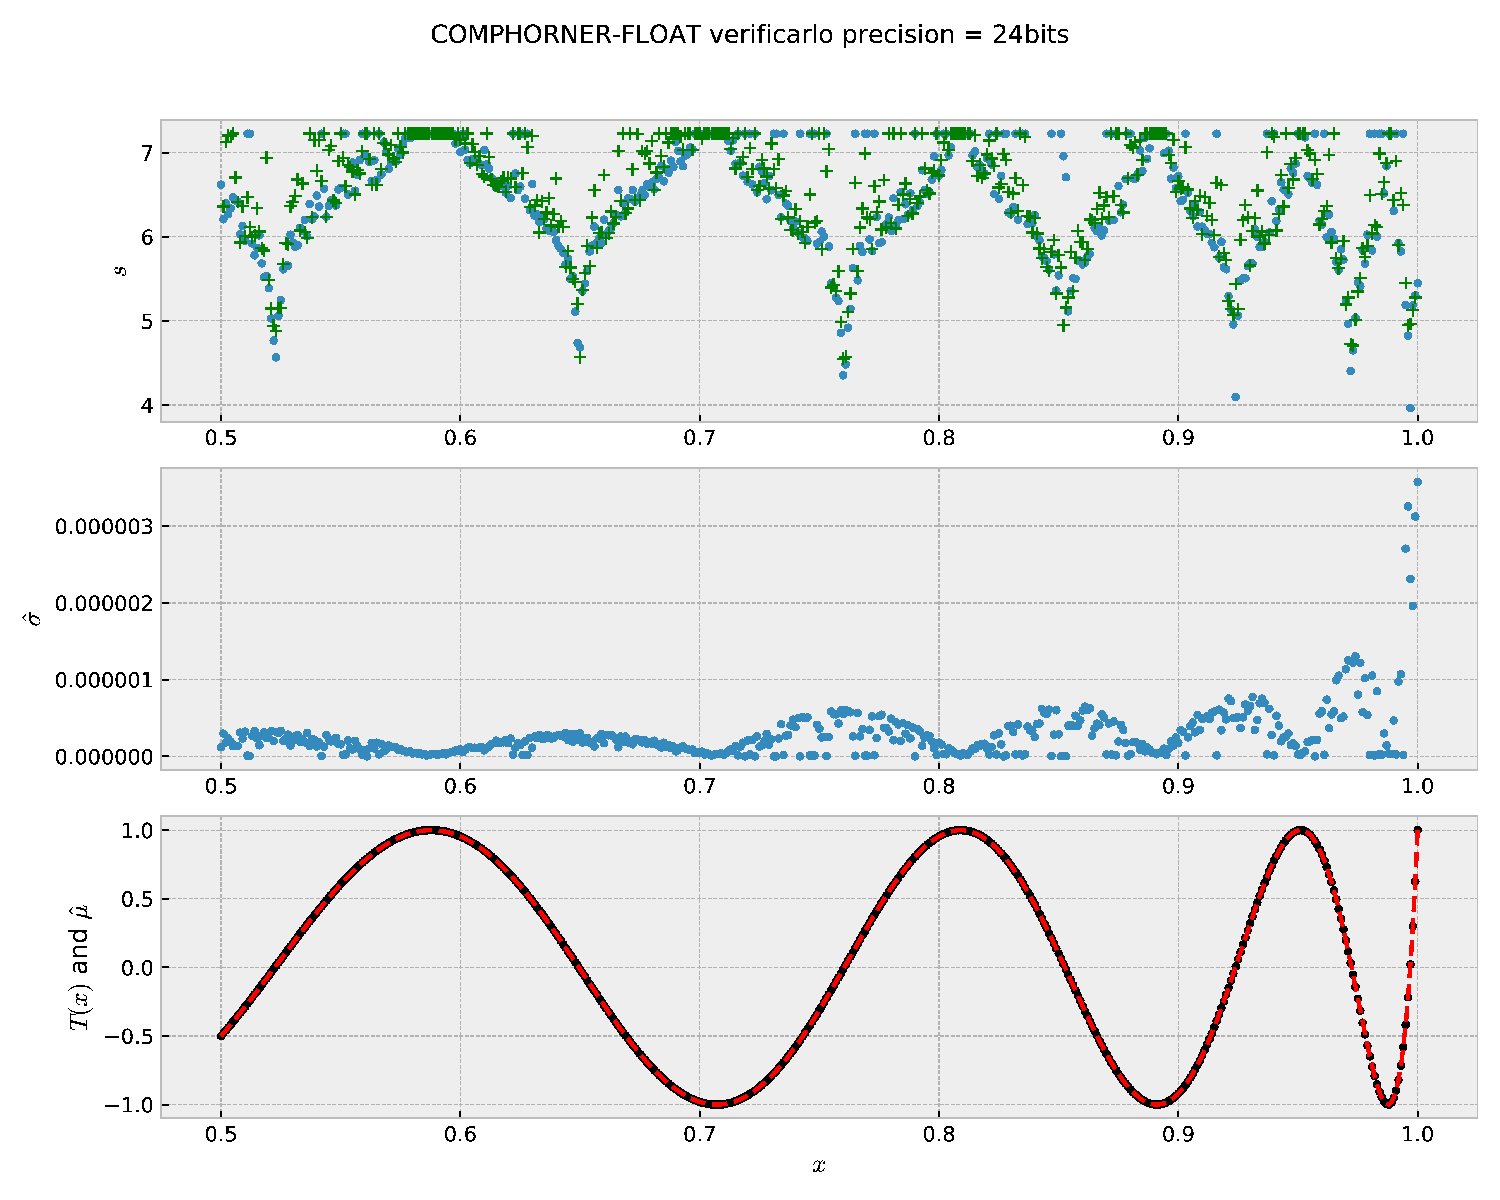
\includegraphics[width=.47\textwidth]{COMPHORNER-FLOAT-24+err.pdf}& 
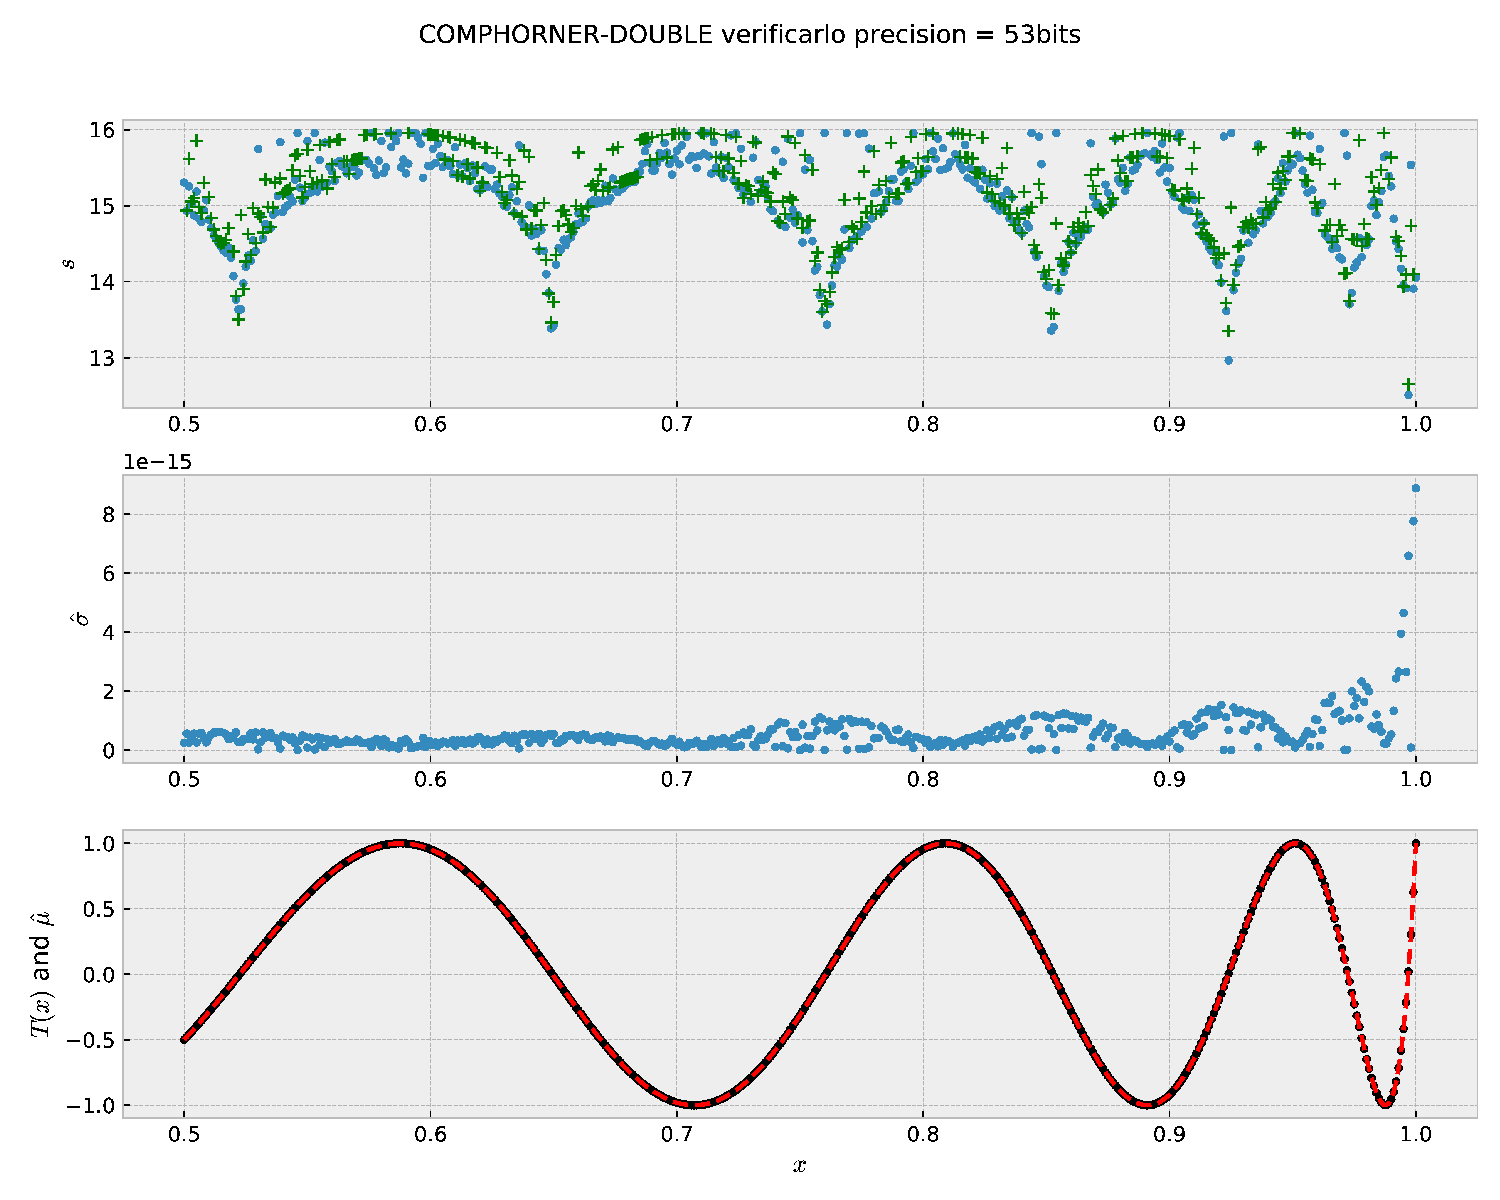
\includegraphics[width=.47\textwidth]{COMPHORNER-DOUBLE-53+err.pdf}\\
\end{tabular}
  \caption{Evaluation of T(x) using Horner and compHorner in single/double (left/right) precision: error estimated by verificarlo (blue), compared to the real error (green)}
  \label{fig:comphornerVerificarlo24_53}
\end{table}


The resulting precision of this approach are given in figures~\ref{fig:comphornerVerificarlo24_53} with verificarlo. 
Filled circles represent the real error value (evaluating in rational arithmetic in Python); circles represent the quality of the result computed in Monte Carlo Arithmetic with Verificarlo~\cite{verrou}.

We can notice on these figures that CompHorner compensate precision losses in double and single precision. We retrieve a behavior similar to the factored form, in particularly for points $T(x)=1$. However, knowing the polynomial's roots for using the Horner scheme is not required.

Out of these plots, we can make two interesting observations.
First, at the cost of an increasing number of operations, (but generally in the same complexity class) it is possible to recover a part (or the full) precision losses. There are algorithms called "accurate" that compute result without loss of precision, by, for example, recursively keeping errors terms until they can not be represented in the final result and such that rounding is correct ({\it e.g.} $accSum$ of S. Hump).

Second, some algorithms, especially in mathematical libraries (libmath, Intel MKL, Intel VML, libeft) used particularity of the floating-point format. By using Monte Carlo Arithmetic, it can be difficult even impossible to analyze them. In the random rounding specific case (as implemented by verificarlo RR mode with a precision length(mantissa)+1), a large amount of compensated algorithms can be analyzed (including compHorner as seen before). In addition, by their design, these algorithms have a proof of their level's precision correctness, which makes their evaluation by empirical methods useless.


